\begin{frame}{Język i struktura}

    \large
    Projekt został napisany w języku \textbf{JAVA} w wersji \textit{OpenJDK~17.0.4} (choć głównie wykorzystuje funkcjonalności dostępne od wersji \textit{OpenJDK 14}).
    
    Klasa \textbf{MinMax} przeszukuje przestrzeń stanów stworzoną z obiektów klasy \textbf{State}.

    Klasa \textbf{Genetic} przeprowadza selekcje na tablicach liczb całkowitych oraz operuje na plikach populacji i plikach ciągów wag w katalogu \textbf{heuristics}.

    % \begin{columns}

    %     \begin{column}{.5\hsize}
    %         \begin{itemize}
    %             \myitem Karl Hasselström \& Jon Åslund, 2001
    %             \myitem Program w SPL wygląda jak szekspirowska sztuka
    %             \myitem Postacie to zmienne
    %             \myitem Wielkość zmiennej zależy wykładniczo od liczby przypisanych do niej komplementów lub przywar
    %         \end{itemize}
    %     \end{column}

    %     \begin{column}{.5\hsize}
    %         \begin{figure}
    %             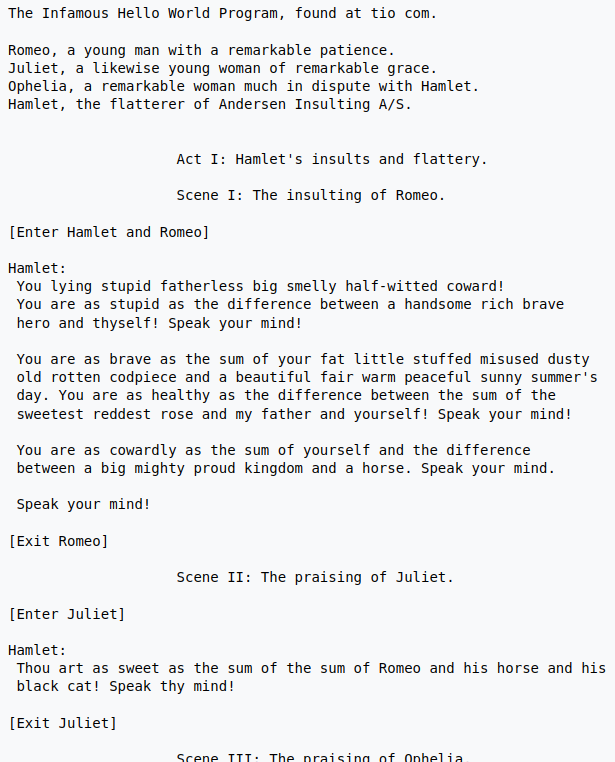
\includegraphics[height=6.3cm]{figures/spl.png}
    %             \caption*{\footnotesize Fragment sztuki ,,Hello World'' {\color{blue} \hyperlink{frame:przypisy}{(5)}}}
    %         \end{figure}
    %     \end{column}

    % \end{columns}

\end{frame}
